\section{NAO Framework}
\label{sec:03_naoFramework}

As stated, a complete code framework exists to address the NAO robots' hardware
in C++ by the \ac{SPL} team \textit{HULKs}.
It is implemented in such manner that \textit{Modules} waits for all input
values (\textit{Dependencies}) which are needed to execute their task.
Modules can be seen as larger coherent operations that fulfills specific purposes.
With the output produced by this Module (\textit{Productions}), successive
Modules can start to perform their cycle.
Due to this sequential process, modules are modifiable independently.
% -------------------------------------------------------------

The robots are able to communicate wirelessly via \ac{UDP} to operate as
multi-agent system.
In the team message protocol, information about the robot states and
knowledge like the believed ball position is exchanged with team mates.
By the \ac{SPL} rules \cite{rules} they are limited to one team message per
robot per second.
However for the whistle localization challenge, not particular specification
about the communication was defined \cite{technical_challenge}.
In order to localize the sound source with multiple robots, results of the
single robot whistle localizations are forwarded to the protocol.
% -------------------------------------------------------------

\subsection{Coordinate Systems}
\label{subsec:03_coordinates}

Two coordinate systems are introduced to consider the whistle sound position.
One for the relative orientation of the source to the robot's head and another
for the absolute position determination in field coordinates.

\Cref{fig:03_naoCoordinate} visualizes the coordinate system of the
robot.
Direction angles $\gamma$ are specified around the z-axis in
mathematically positive direction and range between $-\pi$ and $\pi$.
The direction where the whistle source is believed at by a single robot
will be described as $\gamma$.
% -------------------------------------------------------------

\begin{figure}[ht]
      \centering
      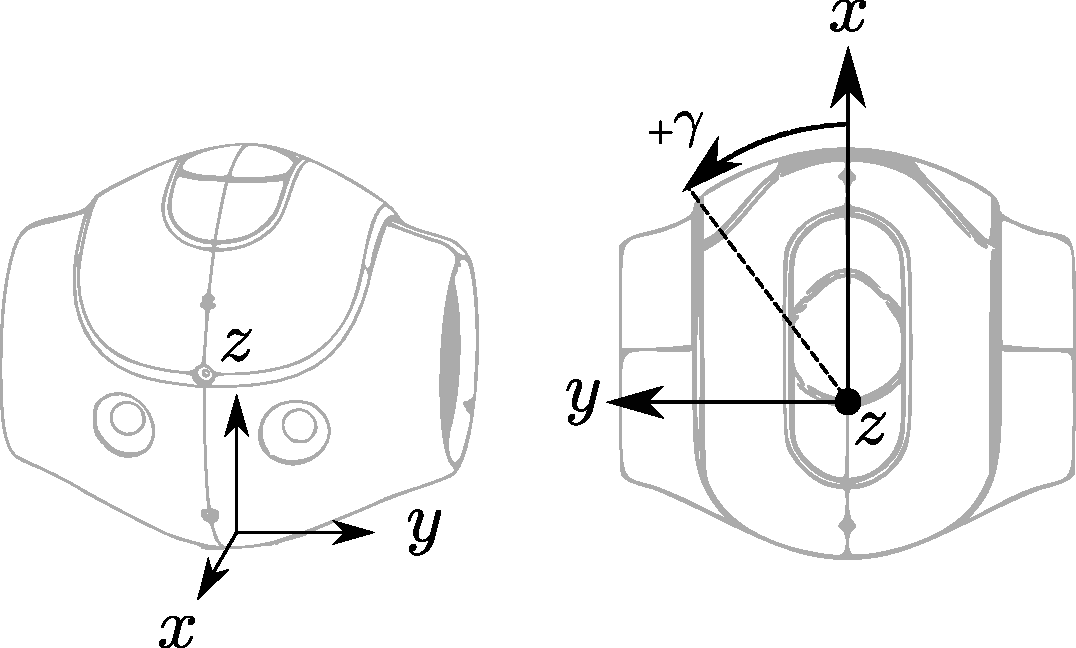
\includegraphics[width=0.60\columnwidth]{figures/nao_coor_both}
      \label{fig:03_naoCoordinate}
      \caption{Coordinate System of NAO's head.}
\end{figure}
% -------------------------------------------------------------

For field coordinates, only the planar case matters in this work.
It is defined as \cref{fig:03_fieldCoordinates} shows.
In game, the robots play into x-direction.
The whistle position of the team filter will be described
in this coordinate system.
% -------------------------------------------------------------
\begin{figure}[ht]
      \centering
      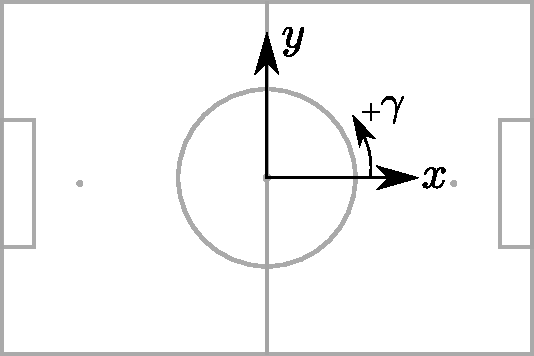
\includegraphics[width=0.50\columnwidth]{figures/field}
      \caption{Field Coordinate System.}
      \label{fig:03_fieldCoordinates}
\end{figure}
% -------------------------------------------------------------

\subsection{Microphones}
\label{subsec:03_microphones}

In \cref{fig:03_micPos} the positions of the four microphones on
the NAO's head that are listed in \cref{tab:03_micPos} with their channel
numbers are outlined.
% channel number from alsa??
% -------------------------------------------------------------
\begin{figure}[ht]
      \centering
      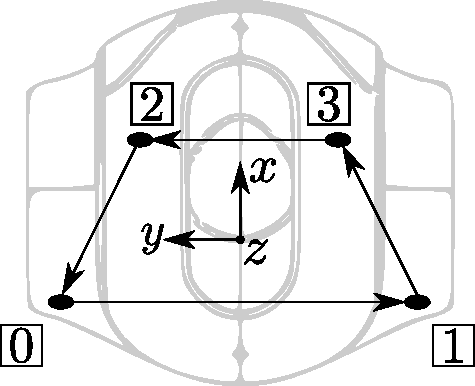
\includegraphics[width=0.35\columnwidth]{figures/mic_pos}
      \caption{Microphone positions on NAO's head.}
      \label{fig:03_micPos}
\end{figure}
% -------------------------------------------------------------
\btline{ht}{1.2}
\btab{|c|c|c|c|}
\hline
Channel & x [\si{\meter}] & y [\si{\meter}] & z [\si{\meter}]\\
\hline
0 & -0,0215 & 0,0558 & 0,0774\\
\hline
1 & -0,0215 & -0,0558 & 0,0774\\
\hline
2 & 0,0206 & 0,0309 & 0,0986\\
\hline
3 & 0,0206 & -0,0309 & 0,0986\\
\hline
\etab
\et{Positions of the microphones on the NAO's head}{03_micPos}
% -------------------------------------------------------------

In this thesis, the next channel is defined as the right adjacent channel.

\subsection{Existing Whistle Detection}
\label{subsec:03_whistleDetection}

% only one channel used
% 1024 fft buffer size in whistle detection.cpp


% -------------------------------------------------------------
\section{Whistle Localization}
\label{sec:03_whistleLocalization}

The procedure of the whistle localization can be briefly outlined by
the following steps:
% -------------------------------------------------------------
\begin{enumerate}
      \item \textbf{Buffer}: the \lstinline!WhistleLocalization! module saves microphone
            data until whistle is detected by the \lstinline!WhistleDetection! module.
      \item \textbf{Single Robot Whistle Localization}: the \lstinline!WhistleLocalization!
            performs the sound source localization algorithm and outputs a
            believed direction angle and additional information if a whistle was detected.
      \item \textbf{Send via Team Message}: angular direction result and additional information
            are sent to other robots by team message.
      \item \textbf{Team Whistle Localization}: wait for results of all agents to be present
            and filter direction information for a final sound position.
\end{enumerate}
% -------------------------------------------------------------


\subsection{Single Robot}
\label{subsec:03_singleRobot}

The direction of a whistle sound source is calculated after a whistle sound was detected
by the existing \lstinline!WhistleDetection! module.
% -------------------------------------------------------------

\subsection{Multi-Agent System}
\label{subsec:03_multiAgend}

% Transform orientation and ray into field coordinates
To agree on a whistle position as multi-agent system, the detected sound source
direction is added into the team message as float.
Depending on the implementation, additional information like distance or
\ac{PSNR} can be appended.

% -------------------------------------------------------------